\chapter{Budúcnosť rozšírenej reality}
\def\thepage{\textit{\arabic{page}}}

Cena zariadení, na ktorých sa dá vytvárať rozšírená realita sa neustále znižuje, zatiaľ čo ich výkon sa rapídne zvyšuje. Pred dvadsiatimi rokmi si bolo možné vyskúšať rozšírenú realitu iba na drahých zariadeniach vo výskumných laboratóriach. Vďaka tomu, že na sprostredkovanú rozšírenú realitu postačí počítač
s kamerou, sa dostupnosť a rozšírenie týchto zariadení zväčšuje. Ľudia si nekupujú zariadenia preto, aby s nimi používali rozšírenú realitu, ale kupujú si zariadenia,
ako sú chytré telefóny a tablety, ktoré dokážu spúšťať rozšírenú realitu, aj keď to nie je ich primárny účel. Počítače sa postupne dostávajú do stále väčšieho množstva chytrých zariadení. Z javu všadeprítomných počítačov (po anglicky \emph{ubiquitus computing}) by mohla rozšírená realita veľa vyťažiť~\cite{Zhou08}.

Rozšírená realita má už dnes množstvo praktických využití, väčšina z nich je ale veľmi špecifická, určená pre úzku skupinu ľudí, alebo veľmi konkrétnu úlohu. Na to, aby sa rozšírená realita v budúcnosti používala viac, je potrebné
vyvinúť všeobecnejšie a praktickejšie aplikácie.

\section{Nové zariadenia}

Veľké pokroky v miniaturizácii len posledné desaťročie umožnili praktické používanie nositeľných počítačov (po anglicky \emph{wearable computers}), teda počítačov, ktoré používateľ nosí na svojom tele tak, ako oblečenie. Koncept okuliarov s rozšírenou realitou existuje už desaťročia, ale ešte donedávna boli všetky helmy vyrobené na tento účel príliš ťarbavé. Počítače, displeje a kamery boli väčšie, nepresnejšie a potrebovali viac energie. Batérie boli ťažšie a zaberali viac priestoru. Helmy s rozšírenou realitou najprv pokrývali celú hlavu, boli ťažké a obmedzovali používateľa pri pohybe. Zo začiatku k~nim bolo potrebné nosiť ruksak, v ktorom sa ukrýval počítač a batérie. Tieto helmy sa postupne zmenšovali, až sa zmenili na okuliare, ale žiadne z nich nedosiahli úroveň, ktorá by mohla dosiahnuť komerčného úspechu a rozšíriť používanie. Pri nositeľných počítačoch je používanie ovplyvnené aj módou. Tieto zariadenia musia vyzerať dobre a ich používatelia sa nesmú cítiť divnými.

\subsection{Google Glass}

Jednými z okuliarov, ktorým by sa mohlo podariť stať sa používanými na verejnosti sú Google Glass. Glass sú futuristické okuliare od Googlu, ktoré majú v ráme zabudovanú malú batériu, počítač, kameru a projektor, ktorý premieta obraz na sklenený hranol pred okom používateľa (sú znázornené na obrázku \ref{glass}). Na rozšírenú realitu nie sú zrovna ideálne, pretože tento hranol je iba v pravom hornom rohu pravého oka, zobrazovacia plocha teda pokrýva iba malú časť zorného pola \cite{Google14-b}. Napriek tomu sa na nich dá rozšírená realita aplikovať — napríklad firma Layar pre ne vytvorila svoju aplikáciu, ktorá používateľovi na domy, na ktoré sa pozerá umiestňuje v prípade, že sú na predaj ikonky a zobrazuje ich stránky v realitných kanceláriach \cite{LayarAR}. Táto aplikácia ale beží iba v rohu užívateľovho zorného pola a domy, ktoré sa v tejto zóne nenachádzajú ignoruje, pretože nemá možnosť na ne ikonky vykresliť. V januári 2015 Google ukončil experimentálnu fázu projektu a prisľúbil, že pracuje na novej verzií.

\begin{figure}[h]
 \centering
 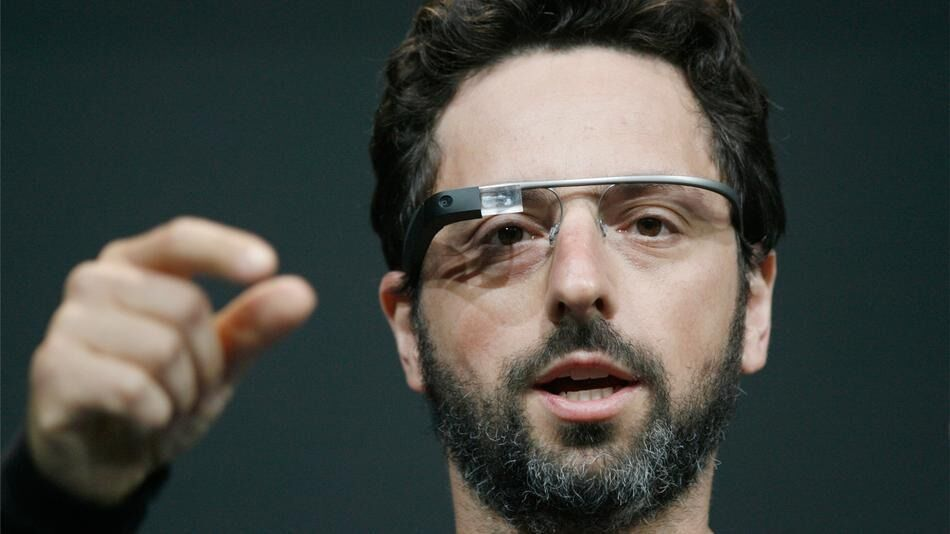
\includegraphics[max width=\textwidth]{pictures/bringlass.jpg}
 \caption{Spoluzakladateľ Google, Sergej Brin demonštruje Google Glass; autor: Kimihiro Hoshino}
 \label{glass}
 \end{figure}

Google Glass nie sú dôležité preto, že by to boli okuliare, ktoré sú dobre uspôsobené na rozšírenú realitu — to nie sú. Sú dôležité preto, že majú potenciál stať sa v budúcnosti komerčne rozšírenou platformou, ktorá môže naštartovať celé nové technologické odvetvie chytrých okuliarov. Práve tak ako chytré telefóny nie sú určené na rozšírenú realitu a napriek tomu sú na ňu používané viac ako zariadenia špeciálne vyvinuté len pre rozšírenú realitu, by sa mohli aj Google Glass, nevyvíjané primárne pre rozšírenú realitu stať budúcou klasickou platformou pre šírenie tejto technológie.

\def\thepage{\arabic{page}}
\subsection{Eyeborg}

Kanaďan Rob Spence prišiel pri nehode o pravé oko. Svojpomocne si skonštruoval protézu s bezdrôtovou kamerou, ktorú odvtedy vylepšuje. Cez toto robotické oko nevidí - zatiaľ sa z neho video odosiela do iného zariadenia, na ktorom sa dá prehrávať. Tento systém obsahuje rozšírenú realitu a dokáže rozoznávať vo videu objekty a manipulovať s~nimi \cite{Eyeborg}. Momentálne musí používateľ pozerať svojim zdravým okom na displej a svalmi v pravej očnej dutine ovláda kameru. Na výskume v oblasti umelého zraku sa pracuje a sú prípady, keď sa podarilo pacientom napojiť signál z kamery na optický nerv a navrátiť im veľmi obmedzené videnie \cite{Dobelle00}. Až sa podobné operácie stanú úplne bežnými, tieto bionické oči budú ideálnou platformou na rozšírenú realitu.

\section{Uchytenie v bežnom živote}

Ukazuje sa, že oblasť je už zrejme dostatočne vyspelá na to, aby bola použiteľná v~bežnej praxi. Nový hardvér umožňuje využívať rozšírenú realitu viac luďom ako kedykoľvek predtým. Jednou z otázok súčastnosti je aj to, či sa tento koncept naozaj presadí v bežnom živote.

V období okolo roku 2009 malo veľké množtvo ľudí svoje prvé chytré mobilné telefóny. V tom čase vzniklo množstvo aplikácií, ktoré využívali rozšírenú realitu rôznymi spôsobmi. Jednou z týchto aplikácií boli napríklad aj slovenské Zlaté Stránky, ktoré na obrazovku telefónu do obrazu z kamery dopisovali názvy firiem na miesta, kde sídlia~\cite{Orgonas10}. Tieto aplikácie sa staly okamžitým hitom, pretože väčšina používateľov si na nich mohla vyskúšať rozšírenú realitu po prvýkrát. Ich popularita však postupne klesla, ako je vidno aj v rebríčkoch mobilných obchodov s aplikáciami, pravdepodobne preto, že praktické využitie a pohodlie používania bolo nízke.

S príchodom chytrých okuliarov dostane rozšírená realita druhú šancu. Najlepšiu použitelnosť a praktickosť by mohli mať napríklad aplikácie s navigáciou. Tieto okuliare sa však zrejme budú musieť rozšíriť za iným cielom, ako napríklad komunikácia a rozšírená realita sa na tomto trende iba zvezie. V oblasti stále existujú veľké sociálne prekážky. Ľudia majú pocit, že používatelia chytrých okuliarov nedávajú pozor a pri~rozhovore sa venujú niečomu inému. Cítiť je aj obavy o súkromie, pretože nevedia, či ich niekto používajúci chytré okuliare tajne nenatáča. Vyskytol sa už aj prípad, kedy používanie Google Glass vyvolalo krčmovú bitku \cite{Gross14}. Mat Honan, jeden z prvých používateľov povedal, že nevie kam ich má nosiť. Nenosí ich do reštaurácie, pretože by to vyzeralo drzo, akoby počas jedla pracoval na telefóne. Nenosí ich do barov, nenosí ich do kina a podobne. Hovorí, že keď má nasadené okuliare na verejnosti cíti sa nekomfortne, pretože ostatní ľudia sú z neho nesvoji a hnevá ich to \cite{Honan13}.

Na druhej strane, v osemdesiatych rokoch sa objavil v spoločnosti takzvaný Walkman efekt. Rozmohli sa hudobné prehrávače Walkman od spoločnosti Sony a ľudia začali na verejnosti nosiť slúchadlá \cite{Honan13}. Mnohých táto situácia hnevala, pretože to považovali za drzé a zdalo sa im, že používatelia Walkmanov nevnímajú svoje okolie. Časom sa prirodzene vyvinuli nové pravidlá etikety hovoriace napríklad o tom, kedy a kde si má človek vytiahnuť slúchadlá z uší. Podobne by sa spoločnosť mohla adaptovať aj na~chytré okuliare.

Je veľmi ťažké predpovedať, ktoré technológie budú úspešné a rozšírené. Doba nositeľných a všadeprítomných počítačov však vyzerá pre rozšírenú realitu ako stvorená.

\pagebreak